%!TEX root=../master_thesis.tex
\chapter{Background}
\label{ch:background}
This chapter contains the necessary information and descriptions of current circumstances to help understand the challenges and reasoning  behind integrating \ac{RS} with Riak Core in place of Consistent Hashing.
First, we give a more detailed description of \ac{RCL}'s implementation of Consistent Hashing.
The following section contains the technical description of \ac{RCL}, a simplified variant of Riak Core.

\section{Consistent Hashing in Riak Core Lite}
\label{sec:riak_core_consistent_hashing}
As Riak Core is an open source implementation of the Dynamo architecture\cite{DeCandia2007} its version of Consistent Hashing is quite similar to Amazon Dynamo's (see \cref{sec:dynamo}).
At the core of the implementation is the ring representing a hash function's hash space.
Here the function in use is SHA-1\cite{Eastlake2001} which results in a hash space of $[0, 2^{160})\subseteq\mathbb{N}$.
Instead of pseudo-randomly distributing nodes on the ring and assigning keys to nodes by smallest distance the ring is split into $n$ partitions of equal size.
To ensure the equal size of all partitions the ring size $n$ has to be set to a power of 2.
The first index of each partition is an index of a virtual node.
The virtual nodes are assigned to physical nodes by \ac{RCL}'s claim algorithm (see \cref{sec:claim}).
Contrary to Amazon's implementation, the physical nodes are assumed to be homogeneous and get assigned the same number of vnodes if it is possible.
To find the node responsible for a given key the key is hashed and the result is placed on the ring.
The node owning the next virtual node index $i$ is responsible for the key.
The $(k+1)$th entry of the preference list for the key can be easily computed by looking at the node owning the index $i + k\cdot2^{160}/n$.

\cref{fig:chash_example} shows an example of a key hashed to a Consistent Hashing ring and how the preference list is constructed.
The ring has a size of 32 with 8 physical nodes.
One can see, that the virtual nodes are responsible for the indices in counter-clockwise direction.
As an example, assume the hash value of ``key'' is owned by node n6.
Then the preference is computed by traversing all predecessor nodes on the ring.
In this case the resulting preference list is [n6, n5, n7, n0, n1, n2, n3, n4, n5].
\begin{figure}
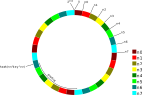
\includegraphics[width=\textwidth]{consistent_hashing_example}
\caption[Consistent Hashing Example]{Consistent Hashing Example.
	Ring with 32 partitions and 8 nodes.}
\label{fig:chash_example}
\end{figure}


\section{Riak Core Lite} 
\label{sec:riak_core_lite}
Riak Core was extracted from the Riak key-value store to enable a simple creation of distributed decentralized systems.
In an attempt to streamline and modularize the concept \ac{RCL}\cite{RiakCoreLiteTeam2020} was created from Riak Core.
One of the biggest motivations to use \ac{RCL} as the system to integrate \ac{RS} with is the simplified structure and shaved off features which leads to a lower potential for complications and errors while still upholding the basic principles of the Dynamo architecture.
As \ac{RCL} is rather a framework for distributed systems than a complete key-value store it's main functionality is the coordination of the nodes in the cluster and navigation of the Consistent Hashing ring.
It does not handle the actual data transfer or replication and instead just returns a plan for the replication in form of a preference list.
The following sections contain an overview of the basic system components and how they interact given some core use cases.

\subsection{System Components}
As the \ac{RCL} System consists of over 40 erlang-modules this sections groups some modules into logical components.
Here the descriptions of the components are on a more abstract level to keep the concepts simple but still enable a discussion of basic system functionalities in \cref{sec:system_procedures}.

\subsubsection{Ring}
	The ring is a central concept in the Dynamo architecture and Consistent Hashing.
	We discussed \ac{RCL}'s implementation of Consistent Hashing and the ring model this component is based on in \cref{sec:riak_core_consistent_hashing}.
	In a cluster every member has its current view of the ring.
	There is only one ring installed per instance, which is only accessible and mutable by this component.
	The ring enables an assignment of keys to nodes and to create the preference list via Consistent Hashing.
	To this end the ring guarantees that for each virtual node at least $N$ predecessor virtual nodes are owned by distinct physical nodes.
	As node failures are assumed as transient in the Dynamo architecture downed nodes are not removed from the ring.
	Instead the Navigation component handles failed nodes by skipping them in the filtered preference list.
	An additional responsibility of the ring is to merge two divergent rings after a network partitioning is fixed.

\subsubsection{Navigation}
	The navigation component enables a user to find the node responsible for a key and creating preference lists.
	It offers to query different kinds of filtered and annotated preference lists.
	For optimization purposes it offers a read-only binary encoding of the current ring with faster access time and lower memory consumption.

\subsubsection{Claim}
	\label{sec:claim}
	Claim handles the rebalancing of the load to nodes when the cluster changes.
	It is used when nodes join, leave or are recognized as down, and when the ring is resized.
	Therefore it is also the entry point of those actions through a stage-plan-commit life cycle in which several changes are staged, the resulting change plan is checked, and the changes are applied to the ring.
	The algorithm keeps the guarantees of the preference list and the ring intact.
	A central aspect of load balancing is to diagonalize the nodes on the ring instead of periodically repeating the same pattern to avoid unfinished patterns at the end of the ring.

\subsubsection{VNode}
	In the context of \ac{RCL} a virtual node represents the combination of the index of the partition on the ring and the owning physical node.
	A member can be a distinct physical machine or an instance on a physical machine.
	Those cases are not distinguished by \ac{RCL} and have to be handle by the system administrator.
	In the component tasks are scheduled and requested at the responsible nodes in an attempt to avoid overloading.
	Those tasks include handling messages sent to the nodes and executing a data handoff to other nodes.
	The virtual node also acts as a behavior definition for those tasks and therefore as the entry point for the application logic when using \ac{RCL}.

\subsubsection{Handoff}
	The handoff implements the concept of transferring data a node previously owned to the node currently owning the keys the data belongs to.
	The handoff component is responsible for creating the connection, creating the correct handoff message and preparing the handoff state a node works on.

\subsubsection{Gossip}
	The gossip protocol is responsible to communicate state updates to other cluster members via a random method that ensures eventual consistency.
	Each node gets assigned tokens periodically.
	As long as a node has tokens it sends the ring to randomly chosen other nodes.
	The gossip component also detects when a ring version changed and triggers the reconciliation in the ring component.

\subsubsection{Eventhandler}
	The eventhandler component allows to install different eventhandlers like one that listens to ring updates.
	Eventhandlers are used by \ac{RCL} internally, however they are also intended to help tailoring the system to the application logic by implementing custom ones.
	Several components are listening to ring update events to trigger procedures.
	This includes starting and registering vnodes or triggering the gossip protocol.

\subsection{System Procedures}
\label{sec:system_procedures}
The system procedures we list here only show a subset consisting of the most basic operations to demonstrate functionality offered by \ac{RCL} and build a ground for comparison to the system adaptions implemented in this thesis.
Any procedure that changes the cluster state, e.g. member status or ring size, have to be applied by the claim's stage-plan-commit cycle which is not explicitly mentioned for those procedures.
In this lifecycle a number of changes is staged via the claimant and premarked in the corresponding place.
Before one can commit the changes, a plan has to be created (see Action \ref{action:plan}, \cref{fig:plan}) and checked if the results are the desired ones.
When committing scheduled changes all changes are applied and the new ring is installed (see Action \ref{action:commit}, \cref{fig:commit}).

\subsubsection{Start Cluster}
When starting the cluster all system processes are started.
This includes starting the ring management system, initializing all virtual nodes and starting the gossip protocol.
When no information about an existing ring can be found on the machine starting the cluster it is assumed this is a new cluster.
Otherwise the ring is installed and the members are queried.
For details see Action \ref{action:start_cluster}, \cref{fig:start_cluster}.

\subsubsection{Join Cluster}
A node in a singleton cluster can join the cluster of another node.
To this end the other node is queried for the remote ring and the membership status of the ring is computed locally.
The ring with the updated members list then is sent via the gossip protocol.
To actually make the new node an owner on the ring the changes have to be planned and committed.
There is no handoff from the joining node to the existing cluster, only in the other direction.
Thus, any keys already stored on the joining node are lost.
For details see Action \ref{action:join_cluster}, \cref{fig:join_cluster}.

\subsubsection{Leave Cluster}
A node can leave the cluster with a call to it's local instance.
This causes the status of the local node to be marked as leaving in the ring.
The new member status is then gossiped to other members in the cluster.
When the claim is executed the next time and the executing node has knowledge of the leaving status the node is not considered for ring ownership and removed.
Leaving is the only ring change that is not applied via the stage-plan-commit life-cycle.
For details see Action \ref{action:leave_cluster}, \cref{fig:leave_cluster}.

\subsubsection{Remove Node}
Removing a node from the cluster causes it to directly hand off all of its data to other nodes.
This leads to a handoff of any sections owned by this node and marking the node invalid.
The status change will lead to the node being excluded from the ring and marked invalid on the next reconciliation.
For details see Action \ref{action:remove_node}, \cref{fig:remove_node}.

\subsubsection{Navigate the Ring}
There are several ways of executing navigation tasks in \ac{RCL}.
Using only the ring one can
\begin{itemize}
	\item find the index of the node responsible for a given key (see Action \ref{action:ring_find_index_for_key}, \cref{fig:ring_find_index_for_key}),
	\item find all indices owned by the local node (see Action \ref{action:ring_find_indices_for_node}, \cref{fig:ring_find_indices_for_node}),
	\item find the node owning a given index (see Action \ref{action:ring_find_node_for_index}, \cref{fig:ring_find_node_for_index}),
	\item compute a simple preference list assuming all nodes are up for a given key (see Action \ref{action:ring_preference_list}, \cref{fig:ring_preference_list}).
\end{itemize}
Via the navigation one can achieve the same results via an optimized structure:
\begin{itemize}
	\item find the index of the section responsible for a given key (see Action \ref{action:chashbin_find_index_for_key}, \cref{fig:chashbin_find_index_for_key}),
	\item compute the position\footnote{The position of a section describes the index of the section on the ring starting from as opposed to the index resulting from the hash function.} of the section responsible for a given key(see Action \ref{action:chashbin_find_partition_index_for_key}, \cref{fig:chashbin_find_partition_index_for_key}),
	\item retrieve the node owning the given index (see Action \ref{action:chashbin_find_ring_index_for_key}, \cref{fig:chashbin_find_ring_index_for_key}),
	\item compute the preference list assuming all nodes are up for a given key (see Action \ref{action:chashbin_preference_list}, \cref{fig:chashbin_preference_list}).
\end{itemize}
Different kinds of active preference lists that only consider up nodes can be computed via the navigation component.
Those include
\begin{itemize}
	\item a plain preference list (see Action \ref{action:get_apl_locally}, \cref{fig:get_apl_locally}).
	\item a preference list in which nodes are annotated as primary or fallback node (see Action \ref{action:get_annotated_apl_locally}, Action \ref{action:get_annotated_apl_locally}).
	\item a preference list only containing primary nodes (see Action \ref{action:get_primary_apl_locally}, \cref{fig:get_primary_apl_locally}).
\end{itemize}

\subsubsection{Resize Ring}
A resize operation can be staged via the claim component.
The ring size must be a power of 2 as otherwise load balancing cannot be achieved.
When a resize is committed special precautions are taken when computing new ownership relations and handoffs to avoid too many unnecessary reassignments and data transfers.
For details see Action \ref{action:resize_ring}, \cref{fig:resize_ring}.

\subsubsection{Handoff}
Nearly all kinds of cluster changes lead to a necessary data transfer.
When such a cluster change is committed via the claim, an entry for scheduled handoffs is added in the updated ring.
The vnode periodically reads these entries and checks for new ones.
When it finds new handoff entries a handoff request is sent to the node handing off data.
When the node is ready to handoff its data a handoff process folding over all stored data items is started by the node.
For details see Action \ref{action:handoff}, \cref{fig:handoff}.
